\section{Introduction}

This technical note presents a detailed analysis of studies around the stray fields of the PS main units.

\subsection{Initial conditions}

In the context of transfer lines, the determination of initial conditions during the construction of the MAD-X lattice model becomes a crucial consideration. While this factor is of less concern for circular machines due to their inherent periodicity, it necessitates explicit specification for linear lattices. Within the Proton Synchrotron (PS), there exist two extraction lines, F16 and F61. One approach to determine the initial conditions at the start of a transfer line, such as F61, is to track the particle within the PS ring and store the beam condition at the junction between the PS and the transfer line for use as initial conditions.

However, this method encounters challenges in the PS where the main components are combined function magnets exhibiting strong stray fields. Complications are further exacerbated due to the necessity of extraction through the magnet's transverse plane, a constraint induced by limited space availability in the straight sections, resulting in a maximal impact from the stray fields. As a result, the beam conditions at extraction remain ambiguous.

To circumvent these challenges, two methodologies are proposed to determine the initial conditions post the stray fields. The first method involves an empirical approach through measurement, which will be discussed in detail in Section \ref{section:Empirical_measurements} \nameref{section:Empirical_measurements}. The second method, on the other hand, resorts to the simulation of the main unit and its associated stray fields, a topic which will be elaborated upon in Section \ref{section:simulation} \nameref{section:simulation}.

\subsection{Stray Fields and Field Maps}
\subsubsection{PS Main Units}

The CERN PS is composed of 100 combined-function Main Units (MU) magnets that produce dipolar and quadrupolar fields simultaneously to provide strong focusing. Each magnet is divided into two half-units with quadrupole gradients of opposite polarity. Half-units are composed of five blocks,
either closed (focusing) or open (defocusing), see Fig. \ref{fig:vector_flow}.
\\

\begin{figure}[H]
\centering
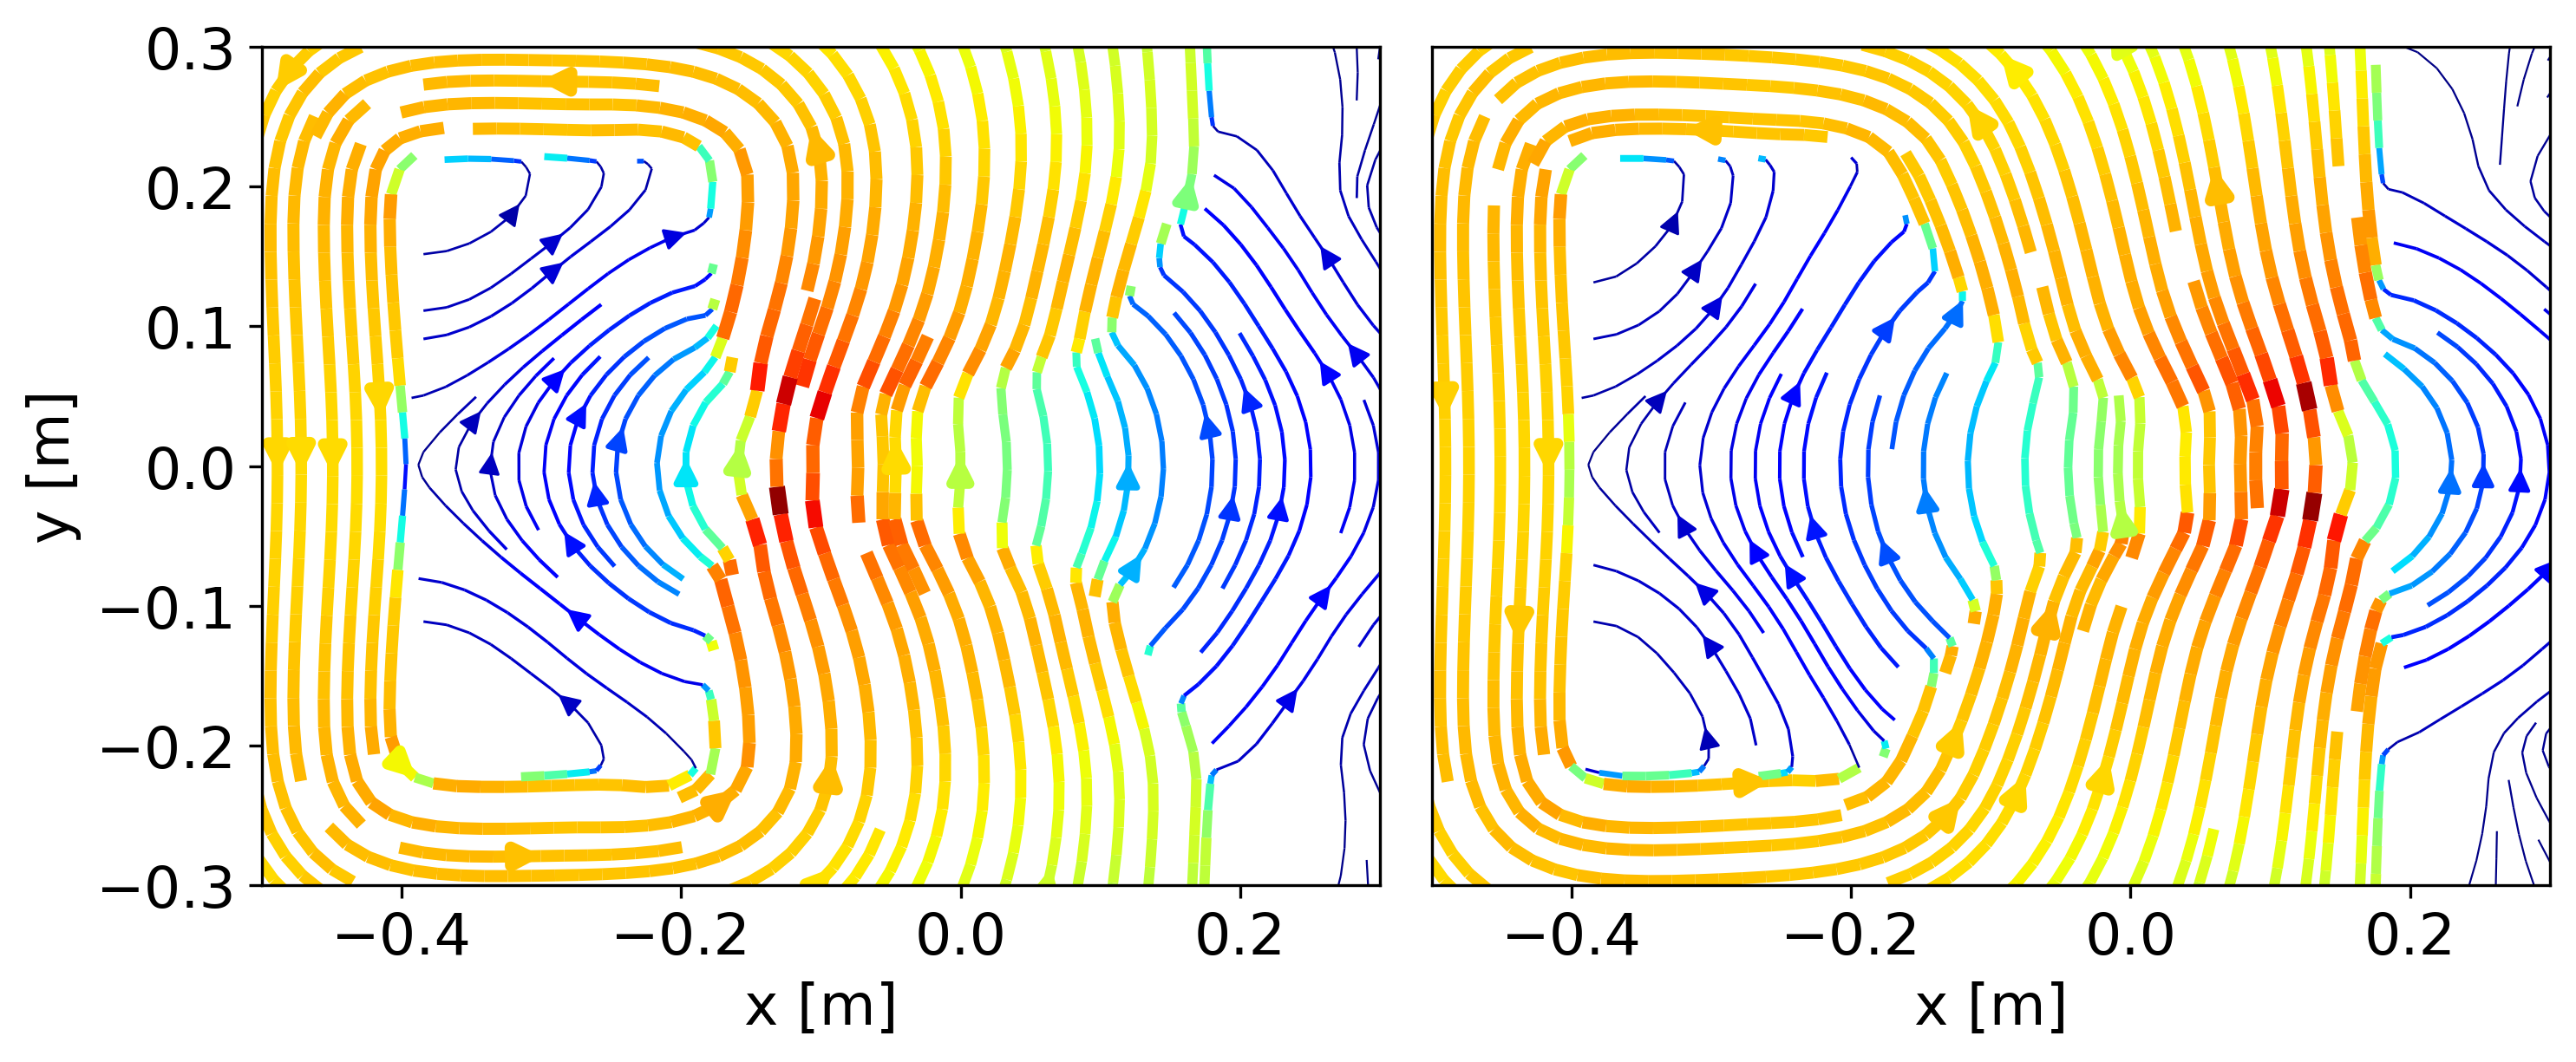
\includegraphics[width=0.7\textwidth]{01_Introduction/images/vector_flow.png}
\caption{Vector flow of an open defocusing block (left) and a closed focusing block (right).}
\label{fig:vector_flow}
\end{figure}

There are four magnets types: R, S, T and U, depending on the arrangement of the half-units (FD or DF) and whether the main coil is on the inside or outside of the ring. Additional coils named the Pole Face Windings (PFW) and Figure-of-eight Loop (F8L) are inserted between the yoke and the vacuum chamber to control the tune and chromaticity. Although the nominal field region of the combined function
magnet extends over a large part of the magnet aperture around the circulating beam orbit, see Fig, \ref{fig:dipole_gradient_components}, the injection and extraction trajectory of the beam travels through strong regions of fringing or stray field. This is a consequence of the PS not being built with straight sections long enough for injection or extraction, forcing the beam to travel through the stray fields of the MUs \cite{risselada_beam_nodate}.
 
\begin{figure}[H]
\centering
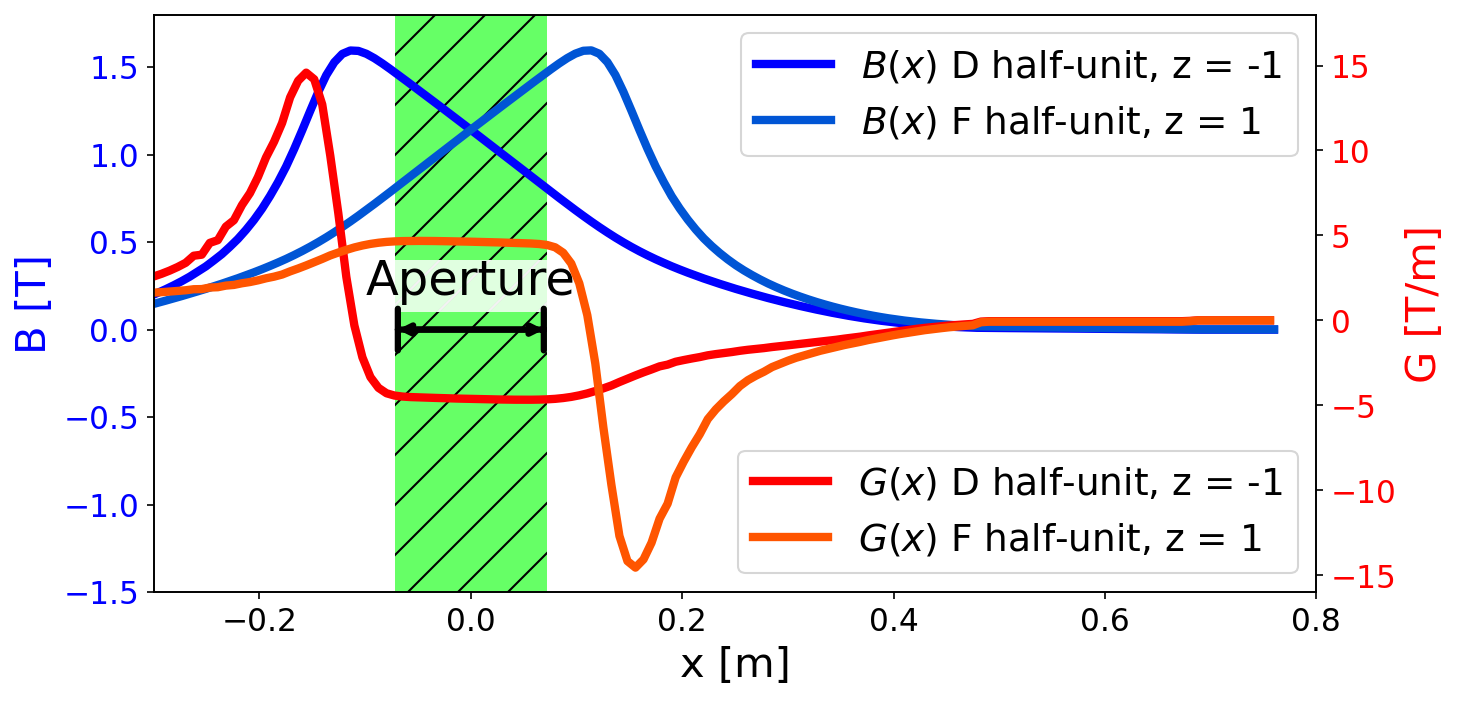
\includegraphics[width=0.7\textwidth]{01_Introduction/images/dipole_gradient_components.png}
\caption{Dipole and gradient component of a PS U-type MU centered in the vertical plane in both half-units at 24 GeV. The green-shaded region of 14.4 cm shows where the gradient is constant to within 5\% of the central and nominal gradient. A width similar to the beam pipe aperture in MU62 of 14.6 cm. Outside this region, the gradient is non-linear and, at its maximum, is almost three-fold higher in amplitude.}
\label{fig:dipole_gradient_components}
\end{figure}

\subsubsection{The OPERA model}

A finite element magnetic model of the PS MU was developed using Cobham's \texttt{Opera-3D}~\cite{noauthor_opera_nodate, anglada_pxmu_hrcwp_nodate} to generate field maps at different energies (different current in the main coils), different PFW, different F8L settings, and for all four magnet types. The model includes the main junction gap of \SI{20}{mm} (a significant source of fringe field) between the two half-units, as well as the mini junctions between open blocks of \SI{9.75}{mm} and \SI{7.75}{mm} between closed blocks. A plane containing the geometry of open and closed yokes is swept in the longitudinal direction, allowing us to maintain a high accuracy of the model and to reduce the computation time. This feature of a single plane also comes with limitations, as it models straight magnets, whilst real magnets have a curvature. The density of the mesh is adjusted so that it has a high resolution in close proximity to the central orbit and at the junctions to capture the fringe fields \cite{anglada_reference_2019}.

An example of a vector field map ($B_x$, $B_y$, $B_z$) in a Cartesian coordinate system ($x$,$y$,$z$) produced by the \texttt{Opera-3D} model is presented in Fig.~\ref{fig:dipole_field}. The transverse displacement of the peak of the vertical dipole field $B_{y}$ along the z-axis corresponds to the switch from one half-unit to the next. The resolution of the field map is high enough to see the mini-junction between the five blocks.

\begin{figure}[!htb]
   \centering
   %trim={<left> <lower> <right> <upper>}
   \includegraphics*[width=0.7\columnwidth, trim={0 2.9cm 0 4.3cm},clip]{01_Introduction/images/dipole_field.png}
   \caption{Dipole field map of a U-type magnet centered in the vertical plane at \SI{24}{GeV}.}
   \label{fig:dipole_field}
\end{figure}

The gradient is calculated from the dipole field component using the following formula:
 
$$ \boldsymbol{G}(x_{j},z) = \frac{\Delta\boldsymbol{B}}{\Delta x} = \frac{\boldsymbol{B}(x_{i+1},z) - \boldsymbol{B}(x_{i},z)}{x_{i+1}-x_{i}} $$
where:
$$ x_{j} = \frac{x_{i+1} + x_{i}}{{2}} $$

\subsubsection{Beam tracking}

Particle tracking through field maps is done using the Boris algorithm that tracks charged particles in EM fields using the discretised equation of motion of the Lorentz force \cite{dutheil_pybttrackersborispy_nodate,qin_why_2013,ripperda_comprehensive_2018}. Field maps were produced for each magnet type at three different energies: injection at \SI{2}{GeV} with \SI{533}{A}, slow extraction to the East Area at \SI{24}{GeV} with \SI{4642}{A}, and extraction to the SPS at \SI{26.4}{GeV} with \SI{5386}{A}. In the following, measurements and tracking studies of injection from the BTP transfer line to the PS and extraction from the PS to the East Area are discussed.

\subsection{Injection via BTP}
As the beam is injected through the BTP transfer line to the PS ring, it passes through the stray fields of the PR.BHT41 T-type MU magnet. The beam traverses mostly through the defocusing half part and feels a non-linear increase in the gradient up to the nominal value in the central orbit; see Fig.~\ref{fig:injection_btp}. Once through MU41, the beam is deflected by the injection septum magnet (PI.SMH42) towards the central orbit. Immediately downstream of the septum, a Secondary Emission Grid (PI.BSG42) is available to measure the position and size of the beam.

\begin{figure}[!htb]
   \centering
   \includegraphics*[width=0.7\columnwidth]{01_Introduction/images/injection_tracking.png}
   \caption{Tracking through MU41 T-type at \SI{2}{GeV}.}
   \label{fig:injection_btp}
\end{figure}

To test the model, measurements of beam position and size on PI.BSG42 were collected as the current provided by the main power supply (POPS) to the MUs was varied. As expected, an increasing current shows that the transverse position of the beam is bent closer towards the inside of the ring by the stronger stray field. Measurements were compared with simulations that tracked a single particle through the \SI{2}{GeV} T-type field map presented in Fig.~\ref{fig:injection_btp_transverse_position}. The tracking simulation overestimates the effect of the stray field because the magnetic model does not yet include the mu-metal shielding wrapped around the injection vacuum pipe. As expected, no deviation was observed in the vertical plane.

\begin{figure}[!htb]
   \centering
   \includegraphics*[width=0.7\columnwidth]{01_Introduction/images/injection_measurement.png}
   \caption{Measurements of the BT3 BTP PS kick response as a function of POPS at PI.BSG42 compared with the OPERA tracking model.}
   \label{fig:injection_btp_transverse_position}
\end{figure}

The current implementation of the stray field in the \mbox{MAD-X}\cite{noauthor_mad_nodate} model is carried out as a sequence of Multipole Field Components (MFC model) expanded along the reference trajectory. A simplified approach with the field components extracted on an injected trajectory assumed as a straight line was compared with the measurements in Fig.~\ref{fig:injection_btp_beam_size}, where the beam size at PI.BSG42 is plotted as a function of the POPS current. We find good agreement in the horizontal plane but a mismatch in the vertical plane. A quadrupole scan was performed on PI.BSG42 and an analysis will tell us whether this is the result of incorrect initial parameters. Similar MFC models for injection and extraction will be created using a Taylor series of the multipole components of the magnetic field about the curved trajectory of the reference particle.

\begin{figure}[!htb]
   \centering
   \includegraphics*[width=0.7\columnwidth]{01_Introduction/images/injection_measurement_beam_size.png}
   \caption{Measurements of the BT3 BTP PS beam size as a function of POPS at PI.BSG42 compared with the MFC model.}
   \label{fig:injection_btp_beam_size}
\end{figure}

\subsection{Extraction to the East Area}
The beam extracted to the East Area is significantly affected by stray fields in multiple main units because the slow extracted trajectory at high energy has a much shallower angle than at injection. As presented in Fig.~\ref{fig:stray field gradients}, the difference in the gradient of MU62 is striking in that the sign of the gradient flips and triples in amplitude. As a result, an increase in the horizontal beam size is expected at the exit of MU62. It is not understood why this magnet was not shimmed in the past to help reduce the effect of the stray field (perhaps because they would significantly impact the central orbit \cite{Zickler:private}), but it is undoubtedly the cause of the optics discrepancy observed during commissioning of the East Area transfer lines in 2021 \cite{huschauer:ipac22-mopost006}.

\begin{figure}[!htb]
   \centering
   \includegraphics*[width=0.7\columnwidth]{01_Introduction/images/gradient_stray_field.png}
   \caption{Gradient seen by the slow extracted beam in the stray field of the few last MUs's focusing half-unit.}
   \label{fig:stray field gradients}
\end{figure}

\subsubsection{Magnetic shims}

To counteract stray fields, magnetic shims are installed in MU16 (fast extraction to SPS) and MU63 (slow extraction to East Area) to homogenise the field by shielding the ejected beam from the non-linear fringe field \cite{zickler_influence_nodate}. In MU16, the shims have different radial positions for each of the five different shims, while in MU63, the vacuum pipe is covered with a constant rectangular shim. In MU62, no shims are installed, where the model predicts the most important stray field effect. In the next step, the shim geometry will be incorporated into the \texttt{OPERA-3D} model, which will significantly increase the computation time of the finite element solver due to the increased complexity of the geometries, but will allow for a more accurate representation of the actual stray fields.

\subsubsection{Measurement of the extracted beam parameters}

Quadrupole scans have been performed to reconstruct the beam parameters in the East Area extraction line. The beam size was measured with Beam instrumentation - TV (BTV) screens as the strength of one or multiple quadrupoles was varied. The initial parameters can be determined empirically by fitting them to a MAD-X simulation against the measurements. BTVs are not ideal instruments for performing these measurements; they saturate at the extraction intensities, and the signal must be fitted with care. Filter wheels have been installed to reduce saturation, allowing for more accurate initial parameter measurement. In addition, a dispersion measurement will be performed to reduce the degrees of freedom of fit.
Kick response measurements have also been carried out. Future studies will compare the initial parameters measured with those predicted by tracking through the field maps in MAD-X.

%\textbf{State clearly the efforts we are going to here to measure the beam parameters that come out of the machine and through the stray fields. State the quad scan technique and challenges with lack of instrumentation but that work continues with BTVs and additional of filter wheels for a comparison with simulation}





\subsection{Previous studies done on the stray fields}

\subsection{Geometry, where do you expect to find stray fields (at injection and extraction F16 and F61)}

\subsection{Shims (no shims in MU62 and shims in MU63)}